\documentclass[tikz, border = 1 cm]{standalone}
\usepackage{tikz}
\usepackage{tkz-euclide}

\begin{document}
    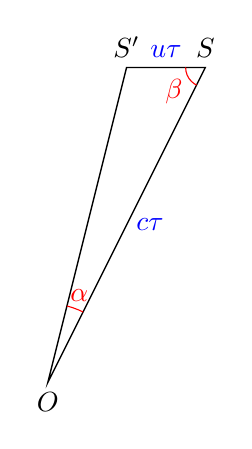
\begin{tikzpicture}
      \tkzDefPoint(0,0){O}
      \tkzDefPoint(1,4){S1}
      \tkzDefPoint(2,4){S2}

      \draw [line width=0.5pt] (O) -- (S1) -- (S2) -- cycle;

      \begin{scope}
        \clip (O) -- (S1) -- (S2) -- cycle;
        
        \draw [red] (O) circle (1);
%        \draw [red] (S1) circle (0.25);
        \draw [red] (S2) circle (0.25);
        \node[red] at (0.4,1.1) {$\alpha$};
        \node[red] at (1.6,3.7) {$\beta$};
      \end{scope}

      \node[below] at (O) {$O$};
      \node[above] at (S1) {$S'$};
      \node[above] at (S2) {$S$};
      \node[right,blue] at (1,2) {$c\tau$};
      \node[above,blue] at (1.5,4) {$u\tau$};
    \end{tikzpicture}

\end{document}
